% !TEX root = Presentation_TheoKoppenhoefer.tex

\input{Preamble_Presentation}

\usepackage[utf8]{inputenc}
% \usepackage{biblatex-beamer}

%%%%% TITLE PAGE

% \subject{}
\title{The Fokker-Planck equation as a gradient flow with respect to the Wasserstein metric}
% \subtitle{A summary of \cite{}}
%\subtitle{Blatt 0}
\author{Theo Koppenhöfer}
% \date{\today}
\date{December 16, 2024}

\setbeamertemplate{bibliography item}{}
\addbibresource{bibliography.bib}

\DeclareBibliographyCategory{image}
\addtocategory{image}{mongeImage, kantorovichImage, candleImage}


% \graphicspath{{../Art/}}
% \graphicspath{{../Plots/}}
\graphicspath{{./Figures/}}
\graphicspath{{./images/}}
\usepackage{import}



\tikzexternaldisable


\usepackage{transparent}


\begin{document}

% \frame[plain]

% Frame 2
% {
%   \usebackgroundtemplate{%
%   {\transparent{0.3}\includegraphics[trim=5cm 5cm 4cm 4cm,width=\paperwidth,height=\paperheight]{../Art/whirl_001_colorised.pdf}}}
% \frame[plain]{\titlepage}
% }

\frame[plain]{\titlepage}


\section{Introduction}

{
  \usebackgroundtemplate{%
  {\transparent{0.3}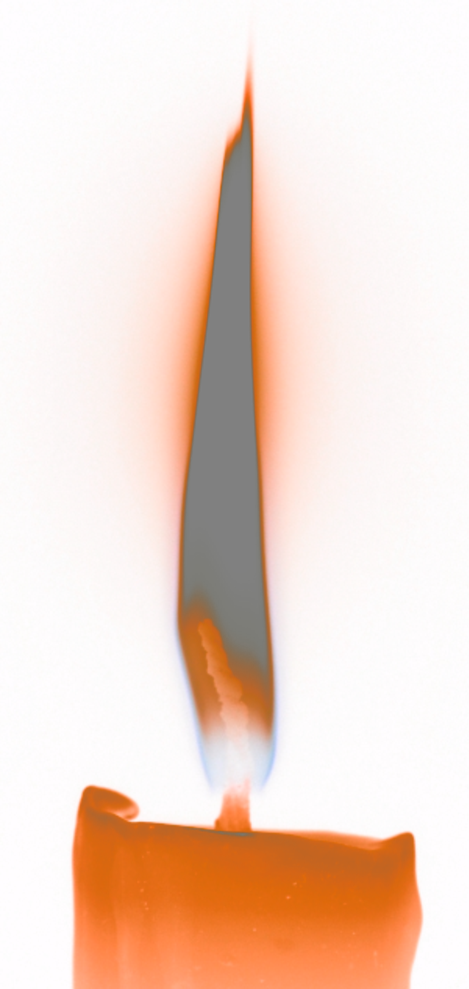
\includegraphics[trim=0cm 8cm 0cm 0cm, height=5cm]{../Images/Candle.pdf}}}
\begin{frame}[plain]
	\begin{center}
		\Large{{The entropy of a closed system never decreases}} \\
    \vspace{1em}
    \footnotesize{{\hfill 2nd law of Thermodynamics (physics convention)}}
	\end{center}
  % \import{Images}{candle.pdf_tex}
\end{frame}
}

\begin{frame}[plain]
	\begin{center}
		\Large{{The heatflow seeks to maximise entropy \\ (with respect to the Wasserstein metric)}} \\
    \vspace{1em}
    \hfill \footnotesize{{Paraphrased summary of \autocite{Otto1998}}}
	\end{center}
\end{frame}


% Frame 3
\frame[plain]{
  \frametitle{Overview}
  \tableofcontents
  }

\subsection{The Fokker-Planck equation}
\begin{frame}
  \frametitle{The Fokker-Planck equation}
  Let $X=\R^d$ and $T=\R_{\geq0}$.
  The \emph{Fokker-Planck equation} is given by
  \begin{align*}
    \partial_t\rho&=\diver\brk*{\nabla\Psi\,\rho}+\frac{1}{\beta}\Delta\rho &\text{ on }X\times T\\
    \rho\brk*{\cdot,0}&=\rho^0 &\text{ on }X
  \end{align*}
  with
  \begin{itemize}
    \item a.e.\ $\rho\colon X\times T\to\R_{\geq0}$, s.t.\ $\rho$ is a probability density at a.e.\ time
    \item smooth potential $\Psi\colon X\to\R_{\geq0}$, s.t.\
      $\abs*{\nabla\psi}\lesssim\Psi+1$ on $X$
    \item parameter $\beta>0$. As in \autocite{Otto1998} set $\beta=1$.
    \item initial probability density $\rho^0\colon X\to\R_{\geq0}$
  \end{itemize}
\end{frame}

\section{Definition of the scheme}
\subsection{The Wasserstein metric}
\subsubsection{Definition}
\begin{frame}
  \frametitle{Wasserstein metric}
  \begin{definition}[Wasserstein metric]
    Let $\mu_i$ be probability measures on $X$ such that
    \begin{align*}
      M\brk*{\mu_i}=\int_X\abs*{x}^2\dif\mu_i<\infty \qquad\text{(finite second moments)}
    \end{align*}
    Define the \emph{set of transport plans} $\Pi\brk*{\mu_1,\mu_2}$ to be the probability measures $p$ on $X\times X$
    such that $p\brk*{\cdot\times X}=\mu_1$ and $p\brk*{X\times\cdot}=\mu_2$ on Borel sets.
    The \emph{Wasserstein metric} is given by 
    \begin{align*}
      d^2\brk*{\mu_1,\mu_2}\coloneqq\inf_{p\in\Pi\brk*{\mu_1,\mu_2}}\int_{X^2}\abs*{x_1-x_2}^2\dif p\brk*{x}
    \end{align*}
  \end{definition}
\end{frame}

\subsubsection{Visualisation}
\begin{frame}
  \begin{figure}
    % \def\svgwidth{10cm}
    \import{Figures}{Wasserstein1.pdf_tex}
    \caption{Motivation of the Wasserstein metric}
  \end{figure}
\end{frame}

\begin{frame}
  \begin{figure}
    \import{Figures}{Wasserstein2.pdf_tex}
    \caption{Motivation of the Wasserstein metric with $\mu_i$ gaussian densities}
  \end{figure}
\end{frame}

\begin{frame}
  \begin{figure}
    \def\svgwidth{7cm}
    \import{Figures}{WassersteinLp.pdf_tex}
    \caption{Difference between Wasserstein and $L^p$ distance}
  \end{figure}
\end{frame}

% \subsubsection{Generalisation}
% \begin{frame}
%   \begin{remark}[Generalisation]
%     More generally one can inspect problems of the type
%     \begin{align*}
%       T_c\brk*{\mu_1,\mu_2}\coloneqq\min_{p\in\Pi\brk*{\mu_1,\mu_2}}\int_{X^2}c\dif p
%     \end{align*}
%     with cost function $c\colon X\times X\to\overline{\R}_{\geq0}$. 
%     This leads to the theory of \emph{optimal transport}.
%     \vspace{0.5cm}
%     \begin{figure}
%     \begin{minipage}[c]{0.4\textwidth}
%       \begin{figure}
%         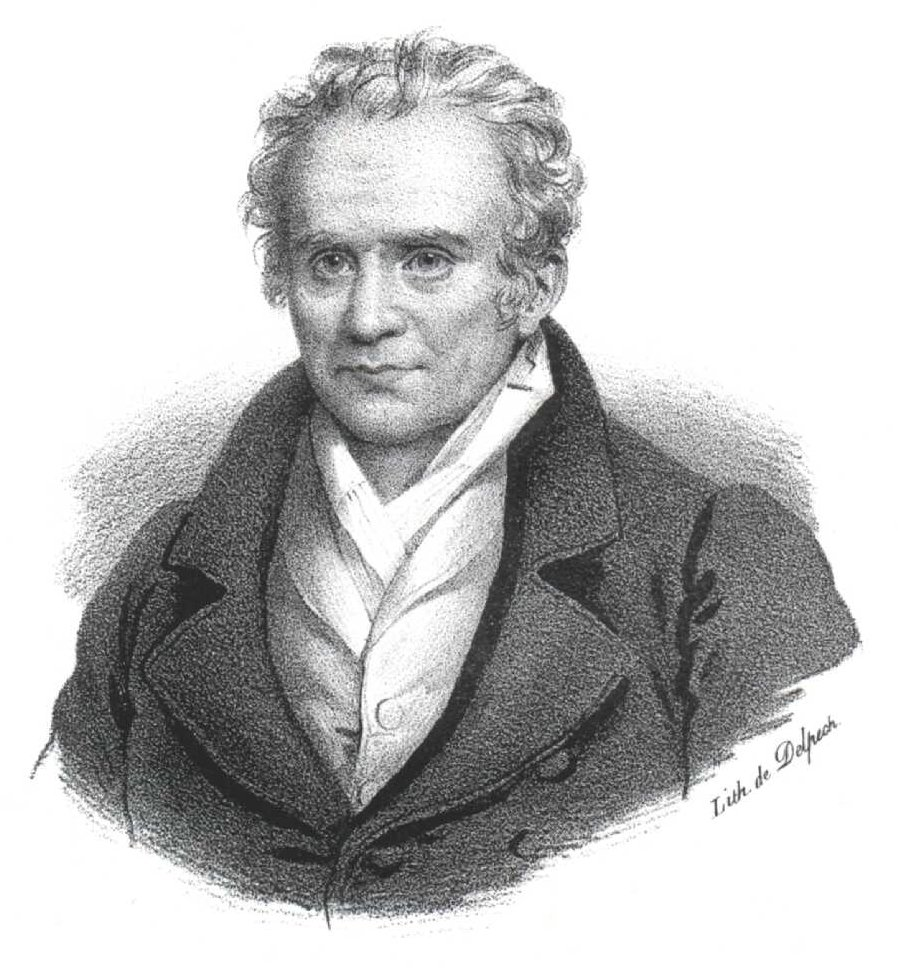
\includegraphics[width=0.5\textwidth]{Gaspard_monge_litho_delpech}
%         \caption{Gaspard Monge}
%       \end{figure}
%     \end{minipage}
%     \hspace{0.5cm}
%     \begin{minipage}[c]{0.4\textwidth}
%       \begin{figure}
%         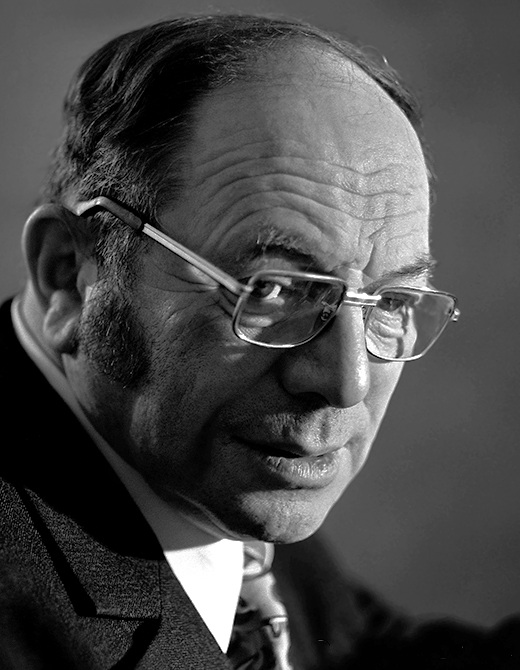
\includegraphics[width=0.4\textwidth]{Leonid_Kantorovich_1975}
%         \caption{Leonid Kantorovich}
%       \end{figure}
%     \end{minipage}
%     \end{figure}
%   \end{remark}
% \end{frame}

\subsection{Time discretisation}
\subsubsection{Definition}
\begin{frame}
  \frametitle{Discretisation in time}
  Define the \emph{(Helmholtz) free energy} as
  \begin{align*}
    \\
    % \annotateEqn[tail=right, tip=below, offsetVert=0.7]{\text{Helmholtz Free Energy}}{F\brk*{\rho}}\coloneqq
    F\brk*{\rho}\coloneqq
    \underbrace{\annotateEqn[tip=above, tail=left, offsetVert=0.1]{\text{internal/potential energy}}{\int_X\Psi\rho}}_{\eqqcolon E\brk*{\rho}}
    +\underbrace{\annotateEqn[tip=above, tail=right, offsetVert=0.1]{Gibbs-Boltzmann  \\ entropy}{\int_X\rho\log\brk*{\rho}}}_{\eqqcolon S\brk*{\rho}}
    \,. % \\
  \end{align*}
  Let $K$ denote the set of probability densities $\rho$ on $X$, s.t.\
  \begin{align*}
    M\brk*{\rho}=\int_X\abs*{x}^2\dif \rho <\infty\,.
  \end{align*}
  Given $\rho^{k-1}$ and $\tau>0$ define the next iterate $\rho^k$ as the minimiser over $K$ of
  \begin{align*}
    \rho\mapsto\frac{1}{2}d^2\brk*{\rho^{k-1},\rho}+\tau F\brk*{\rho}\,.
  \end{align*}
\end{frame}


\subsubsection{Well posedness of the discrete scheme}

\begin{frame}
  \frametitle{Well-posedness}
  \begin{proposition}[Well-posedness, {\autocite[Proposition 4.1]{Otto1998}}]
    Let $\rho_{k-1}\in K$ then there exists a unique minimiser over $K$ of
    \begin{align*}
      \rho\mapsto\frac{1}{2}d\brk*{\rho^{k-1},\rho}^2+\tau F\brk*{\rho}\,.
    \end{align*}
  \end{proposition}
  % \begin{proofs}
  %   Start with uniqueness.
  %   \begin{itemize}
  %     \item The map $\rho\mapsto d^2\brk*{\rho_{k-1},\rho}$ is convex (this makes use of the notion of generalised geodesics and is not trivial, check this!)
  %     \item The function $E\brk*{\rho}=\int_X\Psi\rho$ is linear and $S\brk*{\rho}=\int_X\rho\log\rho$ is convex. Thus 
  %     \item uniqueness follows from convexity
  %   \end{itemize}
  % \end{proofs}
\end{frame}

% \begin{frame}
%   \frametitle{Structure of the proof in {\autocite[Proposition 4.1]{Otto1998}}}
%   \begin{figure}
%     \import{Figures}{proofWellDefined.pdf_tex}
%     % \caption{Structure of the proof in {\autocite[Proposition 4.1]{Otto1998}}}
%   \end{figure}
%   \begin{alert}{Caveat}
%     $F$ is not bounded from below on $K$
%   \end{alert}

%   \begin{alert}{Caveat}
%     '$d^2\brk*{\rho^{k-1},\cdot}$ convex' requires absolutely continuous measures
%   \end{alert}
% \end{frame}

% \begin{frame}
%   \frametitle{Intermezzo: Convexity in Wasserstein spaces}

%   \begin{definition}[Displacement convexity on metric spaces]
%     Let $\brk*{X,d}$ be a metric space.
%     Let $\gamma\colon\brk[s]*{0,1}\to X$ be a uniform speed geodesic, i.e.\
%     locally the shortest path between its endpoints.
%     A function $f\colon X\to\R$ is called \emph{$\gamma$-convex} if $f\circ\gamma$ is convex
%     in the usual sense.
%     It is called \emph{displacement convex} if it is $\gamma$-convex for all such $\gamma$.
%   \end{definition}
%   % \begin{alert}{Caveat}
%   %   The Wasserstein metric is not displacement.
%   %   See e.g.\ \cite[Theorem 7.3.2]{Ambrosio2005}.
%   % \end{alert}
%   \begin{proposition}
%     The Wasserstein metric is displacement convex on $K$.
%   \end{proposition}
%   \begin{alert}{Caveat}
%     The Wasserstein metric is not in general displacement convex.
%     See e.g.\ \cite[Theorem 7.3.2]{Ambrosio2005}.
%   \end{alert}
% \end{frame}


% \begin{frame}
%   \begin{proof}[Well-posedness]
%     We need to show that $F$ is lower-semi continuous.

%     We need to show that $F$ is bounded from below on $K$.
%   \end{proof}
% \end{frame}

\subsection{Interpolation in time}

\begin{frame}
  \frametitle{Interpolation in time}
  Define the step-wise interpolation
  \begin{align*}
    \rho_\tau\brk*{t}
    \coloneqq\sum_k\rho^k\one_{\tau[k,k+1)}\brk*{t}\,.
  \end{align*}
  \vspace*{-0.5cm}
  \begin{figure}
    \def\svgwidth{7cm}
    \import{Figures}{timesteps.pdf_tex}
    \caption{An example for $\rho_\tau$.}
  \end{figure}
\end{frame}

\section{Convergence of the scheme}
\subsection{A priori estimates}

\begin{frame}
  \begin{proposition}[A priori estimates, {\autocite[Theorem 5.1]{Otto1998}}]
    Let $\rho^0\in K$ with $F\brk*{\rho^0}<\infty$.
    Fix an end time $t_1\in T$.
    For all $k_1\tau\leq t_1$ one has 
    % \begin{enumerate}
    %   \item $M\brk*{\rho_\tau}=\int_X\abs*{x}^2\rho_\tau\lesssim 1$\label{en:aPriori_x2}
    %   \item $\int_X \brk*{\rho_\tau\log\brk*{\rho_\tau}}^+\lesssim1$ where $f^+\coloneqq\max\brk*{f,0}$. \label{en:aPriori_log}
    %   \item $E\brk*{\rho_\tau}=\int_X\Psi\rho_\tau\lesssim1$
    %   \item $\sum_{k\leq t_1/\tau}d\brk*{\rho_\tau^{k-1},\rho_\tau^k}^2\lesssim \tau$.
    % \end{enumerate}
    \begin{align*}
      M\brk*{\rho_\tau}=\int_X\abs*{x}^2\rho_\tau&\lesssim 1 &  
      \int_X \brk*{\rho_\tau\log\brk*{\rho_\tau}}^+ &\lesssim 1 \\
      E\brk*{\rho_\tau}=\int_X\Psi\rho_\tau &\lesssim 1 &
      \sum_{k\leq t_1/\tau}d\brk*{\rho_\tau^{k-1},\rho_\tau^k}^2 &\lesssim \tau\,.
    \end{align*}
    where $f^+\coloneqq\max\brk*{f,0}$.
  \end{proposition}
  % \begin{proof}[Idea of proof]
  %   See \autocite[Theorem 5.1]{Otto1998} for details.
  %   The main ideas are
  %   \begin{itemize}
  %     \item Obtaining a telescopic sum from $ $
  %     \item Using that $S\brk*{\rho}\geq-C\brk*{M\brk*{\rho}+1}^\alpha$ for some $\alpha<1$.
  %     \item Using that $ d$
  %   \end{itemize}
  % \end{proof}
% \end{frame}

% \subsection{Weak convergence}

% \begin{frame}
  % \frametitle{Weak convergence of the scheme}
  \begin{corollary}[Weak convergence, {\autocite[Theorem 5.1]{Otto1998}}]
    Let $\rho^0\in K$ with $F\brk*{\rho^0}<\infty$.
    Then for a subsequence $\rho_\tau\rightharpoonup\rho$ weakly in $L^1\brk*{\brk*{0,t_1}\times X}$ for all finite end times $t_1$.
    Additionally $\rho\in K$ for a.e.\ time and $M\brk*{\rho},E\brk*{\rho}\in L^\infty\brk*{(0,t_1)}$.
  \end{corollary}
  % \begin{proof}[Proof of weak convergence]
  %   $\rho_\tau$ is bounded in $L^1\brk*{X\setminus B_1}$ since $M\brk*{\rho_\tau}\lesssim1$
  %   and is bounded in $L^1\brk*{B_1}$ since $\int_X\brk*{\rho_\tau\log\rho_\tau}^+\lesssim1$.
  % \end{proof}
\end{frame}


% \begin{frame}
%   One can show with these estimates
%   \begin{proposition}[Improved convergence, {\autocite[Theorem 5.1]{Otto1998}}]
%     \rho_\tau\brk*{t}\to\rho\brk*{t}
%   \end{proposition}
%   weakly in $L^1\brk*{X}$ for all times $t$.
% \end{frame}

\subsection{Limit solves Fokker-Planck}

\begin{frame}
  \frametitle{Taking the limit $\tau\to0$}
  \begin{proposition}[$\rho$ solves weak Fokker-Planck, {\autocite[Theorem 5.1]{Otto1998}}]
    Let $\rho_\tau\rightharpoonup \rho$ weakly in $L^1\brk*{\brk*{0,t_1}\times X}$ for all finite times $t_1$.
    Then $\rho$ solves the weak Fokker-Planck equation. 
  \end{proposition}
  Classical arguments (e.g.\ convolution with a heat kernel)
  then yield that this solution is strong, smooth and unique.
  See \cite[Theorem 5.1]{Otto1998}.
  % \begin{theorem}[]
  %   Let $\rho^0\in K$ with $F\brk*{\rho^0}<\infty$.
  %   Then $\rho_\tau$
  % \end{theorem}
  % \begin{proof}[Idea of proof]
  %   Convolution with the heat kernel.
  % \end{proof}
  % Set $\beta=1$ in the Fokker-Planck equation.
\end{frame}


\begin{frame}
  \begin{proofs}
    The proof comes from \autocite[Theorem 5.1]{Otto1998}.
    The main idea is to perturb around $\rho^k$.
    For this let $\Phi_s\colon X\to X$ be such that
    \begin{wrapfigure}{r}{0.4\textwidth}
      \def\svgwidth{0.5\textwidth}
      % \hspace*{-0.5cm}
      \import{Figures}{potentialWell.pdf_tex}
      % \vspace*{-9cm}
      \caption{The situation at hand}
    \end{wrapfigure}
    \begin{equation*}
      \begin{aligned}
        \partial_s\Phi_s&=\nabla\zeta \\
        \Phi_0&=\Id
      \end{aligned}
      \qquad\qquad\text{(flux)}
    \end{equation*}
    for $\nabla\zeta\in C_0^\infty\brk*{X;X}$.
    Define the push forward
    $$\rho_s\coloneqq J\brk*{\Phi_s}\,\rho^k\circ\Phi_s^{-1}$$
    where $J\brk*{f}\coloneqq\det\nabla f$ is chosen such that the pertubation remains in $K$.
  \end{proofs}
\end{frame}


\begin{frame}
  \begin{proofs}
    We perturb
    \begin{align*}
      \\
      0&\annotateEqn[offsetVert=0.3]{$\rho^k\text{ minimises }\rho\mapsto\frac{1}{2\tau}d^2\brk*{\rho^{k-1},\rho}+F\brk*{\rho}$}{\leq}
      \frac{1}{s}\brk*{\brk*{\frac{1}{2\tau}d^2\brk*{\rho^{k-1},\rho_s}+F\brk*{\rho_s}}-\brk*{\frac{1}{2\tau}d^2\brk*{\rho^{k-1},\rho^k}+F\brk*{\rho^k}}} \\ \\
      &\annotateEqn[offsetVert=0.3]{$F=E+S$}{=}\underbrace{\frac{1}{2\tau s}\brk*{d^2\brk*{\rho^{k-1},\rho_s}-d^2\brk*{\rho^{k-1},\rho^k}}}_{\eqqcolon{\cyan\brk*{I}^k_s}}+ \\
      &\qquad+\underbrace{\frac{1}{s}\brk*{E\brk*{\rho_s}-E\brk*{\rho^k}}}_{\eqqcolon{\magenta\brk*{II}^k_s}}
      +\underbrace{\frac{1}{s}\brk*{S\brk*{\rho_s}-S\brk*{\rho^k}}}_{\eqqcolon{\lime\brk*{III}^k_s}}
    \end{align*}
  \end{proofs}
\end{frame}

\begin{frame}
  \begin{proofs}
    We inspect the pertubation of the internal energy
    \begin{align*}
      {\magenta\brk*{II}^k_s}&=\frac{1}{s}\brk*{E\brk*{\rho_s}-E\brk*{\rho^k}} \\ \\
      &\annotateEqn[offsetVert=0.3]{$E\brk*{\rho}=\int_X\Psi\rho$ and $\rho_s=J\brk*{\Phi_s}\rho^k\circ\Phi_s^{-1}$}{=}
      \frac{1}{s}\int_X\Psi\,\brk*{J\brk*{\Phi_s}\,\rho^k\circ\Phi_s^{-1}-\rho^k} \\  \\
      &\annotateEqn[offsetVert=0.3]{change of variables}{=}\int_X\frac{1}{s}\brk*{\Psi\circ\Phi_s-\Psi\circ\Phi_0}\rho^k \\ \\
      &\annotateEqn{$\partial_s\Phi_s=\nabla\zeta$}{\xrightarrow{s\to0}}  \int_X\nabla\Psi\cdot\nabla\zeta\,\rho^k
    \end{align*}
  \end{proofs}
\end{frame}

\begin{frame}
  \begin{proofs}
    The pertubation of the Gibbs-Boltzman entropy becomes
    \begin{align*}
      {\lime\brk*{III}^k_s}&=\frac{1}{s}\brk*{S\brk*{\rho_s}-S\brk*{\rho^k}} \\ \\
      &\annotateEqn[offsetVert=0.3]{$S\brk*{\rho}=\int_X\rho\log\brk*{\rho}$ and $\rho_s=J\brk*{\Phi_s}\rho^k\circ\Phi_s^{-1}$}{=}
      \frac{1}{s}\int_X J\brk*{\Phi_s}\rho^k\circ\Phi_s^{-1}\log\brk*{J\brk*{\Phi_s}\rho^k\circ\Phi_s^{-1}}-
      \rho^k\log\brk*{\rho^k} \\ \\
      &\annotateEqn[offsetVert=0.3]{change of variables}{=}\frac{1}{s}\int_X \rho^k\brk*{\log\brk*{J\brk*{\Phi_s}\rho^k}-\log\brk*{\rho^k}} \\
      &=\int_X \rho^k\frac{1}{s}\brk*{\log\brk*{\det\nabla\Phi_s}-\log\brk*{\det\nabla\Phi_0}} \\ \\
      &\annotateEqn{Jacobi's formula and $\partial_s\Phi_s=\nabla\zeta$}{\xrightarrow{s\to0}}\int_X \rho^k\diver\nabla\zeta
      = \int_X\rho^k\Delta\zeta
    \end{align*}
  \end{proofs}
\end{frame}

\begin{frame}
  \begin{proofs}
    % The following is central to why one considers Wasserstein metrics:
    For the pertubation of the Wasserstein term let $p$ be such that
    \begin{align*}
      d^2\brk*{\rho^{k-1},\rho^k}=\int_{X^2}\abs*{x_1-x_2}^2\dif p\brk*{x}\,.
    \end{align*}
    Define the push forward measure $p_s\in\Pi\brk*{\rho^{k-1},\rho_s}$ through
    \begin{align*}
      \int_{X^2}f\brk*{x_1,x_2}\dif p_s=\int_{X^2}f\brk*{x_1,\Phi_s\brk*{x_2}} \dif p
    \end{align*}
    for all measurable $f\colon X^2\to\R$.
    % $$J\brk*{\Phi_s\brk*{x_2}}p\brk*{x_1,\Phi_s^{-1}\brk*{x_2}}\in\Pi\brk*{\rho^{k-1},\rho_s}$$
    % Since
    % \begin{align*}
    %   \int_XJ\brk*{\Phi_s\brk*{x_2}}p\brk*{x_1,\Phi_s^{-1}\brk*{x_2}}\dif x_2&=\rho^{k-1}\brk*{x_1} \\
    %   \int_XJ\brk*{\Phi_s\brk*{x_2}}p\brk*{x_1,\Phi_s^{-1}\brk*{x_2}}\dif x_1&=J\brk*{\Phi_s}\rho^k\circ\Phi_s^{-1}\brk*{x_2}=\rho_s\brk*{x_2} \\
    % \end{align*}
  \end{proofs}
  % \begin{remark}
  %   We will see that the inequalities are equalities in the limit.
  % \end{remark}
\end{frame}

\begin{frame}
  \begin{proofs}
    so we obtain
    \begin{align*}
      \tau{\cyan\brk*{I}^k_s}&=\frac{1}{2s}\brk*{d^2\brk*{\rho^{k-1},\rho_s}-d^2\brk*{\rho^{k-1},\rho^k}} \\
      &\leq \frac{1}{2s}\brk*{\int_{X^2}\abs*{x_2-x_1}^2\dif p_s-\int_{X^2}\abs*{x_2-x_1}^2\dif p} \\ % \\
      % &\annotateEqn[offsetVert=0.3]{Change of variables}{=}
      &= \frac{1}{2s}\int_{X^2}\brk*{\abs*{\Phi_s\brk*{x_2}-x_1}^2-\abs*{\Phi_0\brk*{x_2}-x_1}^2}\dif p \\
      &\xrightarrow{s\to0}\int_{X^2}\brk*{x_2-x_1}\cdot\nabla\zeta\dif p \\ \\
      % \limsup_{s\to\infty}\tau{\cyan\brk*{I}^k_s}&\leq\int_{X^2}\brk*{x_2-x_1}\cdot\nabla\zeta\dif p \\ \\
      &\annotateEqn[offsetVert=0.3]{Taylor}{=}\int_{X^2}\zeta\brk*{x_1}-\zeta\brk*{x_2}\dif p
      +\bigO\brk*{\frac{\abs*{\nabla^2\zeta}_{L^\infty}}{2}\int_{X^2}\abs*{x_2-x_1}^2\dif p} \\
      &=\int_{X}\zeta\brk*{\rho^{k-1}-\rho^k} +\bigO\brk*{d^2\brk*{\rho^{k-1},\rho^k}} \\
    \end{align*}
  \end{proofs}
\end{frame}


\begin{frame}
  \begin{proof}
    Putting things together for finite time $T=\brk[s]*{0,t_1}$ % and 
    \begin{align*}
      0&\leq\int_T\limsup_{s\to0}\sum_k\brk*{{\cyan\brk*{I}^{k+1}_s}+{\magenta\brk*{II}^{k+1}_s}+{\lime\brk*{III}^{k+1}_s}}\one_{\tau[k,k+1)}\brk*{t} \\
      &\leq \int_{T\times X}{\cyan\zeta\frac{\rho_\tau-\rho_\tau\brk*{\cdot+\tau}}{\tau}}
      +{\magenta\nabla\Psi\cdot\nabla\zeta\,\rho_\tau}
      + {\lime\rho_\tau\Delta\zeta} \\
      &\qquad+{\cyan\abs*{T}\bigO\brk*{\sum_{k\leq t_1/\tau}d^2\brk*{\rho^{k-1},\rho^k}}} \\
      &=\int_{T\times X}\rho_\tau\brk*{\frac{\zeta-\zeta\brk*{\cdot-\tau}}{\tau}+\nabla\Psi\cdot\nabla\zeta+\Delta\zeta}
      -\int_{X}\rho^0\zeta\brk*{0,\cdot} +\dots\\ \\
      % &\qquad+\abs*{T}\bigO\brk*{\sum_{k\leq t_1/\tau}d^2\brk*{\rho^{k-1},\rho^k}}
      %  \\
      &\annotateEqn{A priori estimate}{\xrightarrow{\tau\to0}}
      \int_{T\times X}\rho\brk*{\partial_t\zeta-\nabla\Psi\cdot\nabla\zeta+\Delta\zeta}-\int_{X}\rho^0\zeta\brk*{0,\cdot}
    \end{align*}
    for all $\zeta\in C_0^\infty\brk*{\R\times X}$.
    This means that $\rho$ fulfills the weak Fokker-Planck equation.
    % Using symmetry of $\zeta\leftrightarrow-\zeta$ one sees that $\rho$ solves the weak Fokker-Planck equation
    % \begin{align*}
    %   \int_{X\times T}\rho\brk*{\partial_t\zeta-\nabla\Psi\cdot\nabla\zeta+\Delta\zeta}=\int_X\rho_0\zeta\brk*{0,\cdot}
    %   \text{ for all }\zeta\in C_0^\infty\brk*{\R\times X}
    % \end{align*}
    % Now for $\tau\to0$ it follows that
    % \begin{align*}
    %   \abs*{d^2\zeta}_\infty d^2\brk*{\rho^{k-1},\rho^k}\to0
    % \end{align*}
    % and
  \end{proof}
\end{frame}

% \begin{frame}
%   \begin{proofs}
%     The main idea is: show that the weak equation
%     holds.
%   \end{proofs}
% \end{frame}

\section{Summary}

\begin{frame}
  \frametitle{Summary}
  % \begin{itemize}
  %   \item We have defined the Wasserstein metric
  %   \item 
  % \end{itemize}
  We have (in some sense) $\rho_\tau\to \rho$ where
  \begin{itemize}
    \item $\rho$ solves the Fokker-Planck equation $\partial_t\rho=\diver\brk*{\nabla\Psi\,\rho}+\Delta\rho$
    \item $\rho_\tau\brk*{t}=\sum_k\rho^k\one_{\tau[k,k+1)}\brk*{t}$
    \item $\rho^{k}$ minimises $\frac{1}{2}d^2\brk*{\rho^{k-1},\cdot}+\tau F$ over $K$
    \item $F$ is the (Helmholtz) free energy $\int_X\Psi\rho+\int_X\rho\log\brk*{\rho}$
    \item $d$ is the Wasserstein metric given by $d^2\brk*{\mu_1,\mu_2}=\inf_{p\in\Pi\brk*{\mu_1,\mu_2}}\int_{X^2}\abs*{x_1-x_2}^2$
  \end{itemize}
\end{frame}

% {
%   \usebackgroundtemplate{%
%   {\transparent{0.6}\includegraphics[trim=5cm 3cm 3cm 5cm,width=\paperwidth,height=\paperheight]{../Art/circular_001_colorised.pdf}}}
\begin{frame}[plain]
	\begin{center}
		\Large{{Thank you for your attention.}}
	\end{center}
\end{frame}
% }

\section{Sources}

\begin{frame}[allowframebreaks]
	\frametitle{Sources}
	\nocite{*}
  
	% \bibliographystyle{plain}
	% \setbeamertemplate{bibliography item}[text]
  % \setbeamertemplate{bibliography item}{\insertbiblabel}
	% \bibliography{bibliographyFile}
	\printbibliography[notcategory=image]
\end{frame}

\begin{frame}[allowframebreaks]
  \frametitle{Image Credits}
  \printbibliography[category=image]
\end{frame}


% \frame[plain]

\end{document}
